\section{Galaxy Classification}


In this section we will attempt to implement a logistic regression algorithm to classify galaxies into two classes, ellipticals and spirals, using four parameters:

\begin{itemize}
    \item $\kappa_{\mathrm{co}}$, which indicates how much a galaxy is dominated by ordered rotation
    \item A color estimate (higher is redder, and therefore contains older stars)
    \item A measure of how extended the galaxy is
    \item Flux of an emission line tracing the star formation rate
\end{itemize}

We start by preprocessing all of the features by scaling them to have zero mean and unit standard deviation. This is implemented for each feature $f_i$ separately as

\begin{equation}
    f_{i, \mathrm{scaled}} = \frac{f_i - \mu_i}{\sigma_i}
\end{equation}

To get a sense of how each of our features is distributed, we plot their histograms in Figure \ref{fig:feat_dist}, and present the first ten samples below.

\lstinputlisting[caption={Scaled feature values for the first ten entries of the galaxy dataset}, lastline=10]{results/scaled_features.txt}
\lstinputlisting[caption={Code to make the histograms in Figure \ref{fig:feat_dist}}, linerange={15-36}]{plotting.py}
\lstinputlisting[caption={Code for the feature preprocessing and plotting.}, linerange={6-36}]{classification.py}

\begin{figure}
    \centering
    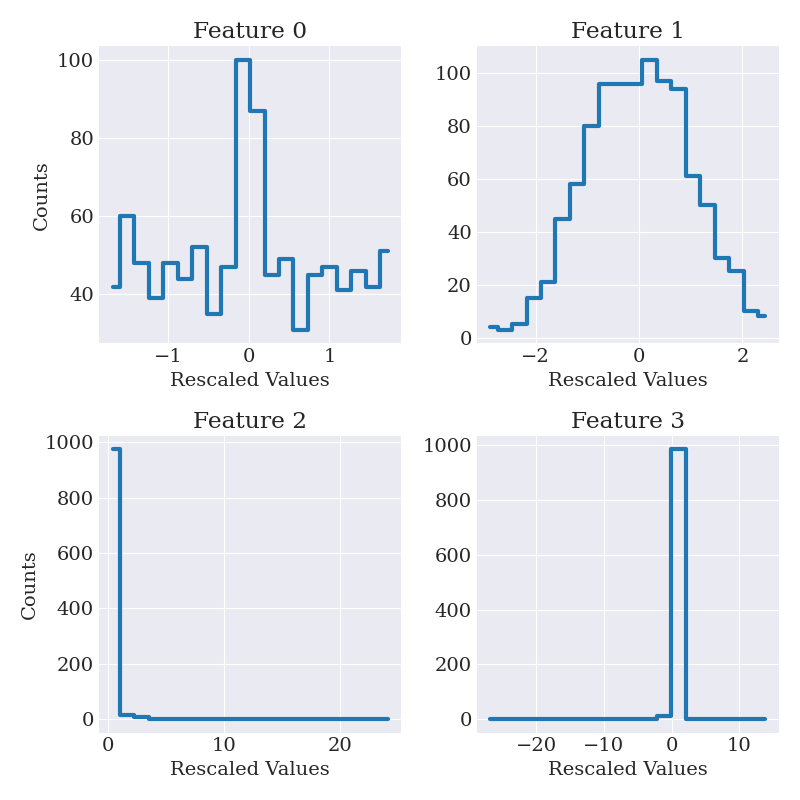
\includegraphics[width=0.8\textwidth]{results/scaled_features_dist.png}
    \caption{Distributions of the scaled features used for the classification algorithms in this section.}
    \label{fig:feat_dist}
\end{figure}

It is immediately noticable that while most values for features 2 and 3 lie around 0, there are outliers at extremely high values. This is less true for feature 0 which shows a peak at 0 and has a relatively constant distribution in its wings. Feature 1 appears to be nicely distributed close to a Gaussian. Due to the few outliers in features 2 and 3 we will limit ourselves to the 2\% and 98\% percentiles for plotting in the rest of this work to better highlight the variations in the regions where the bulk of the datapoints reside. Ofcourse we do not discard these points for the training process.

\subsection{Two Feature Combinations}


We begin by investigating how well the logistic regression algorithm is able to predict the galaxy class if it is only provided with two of the four available features. We do this by running the algorithm by each of the six possible combinations of two features and investigating the resulting loss values. In each case we also include a bias feature consisting of only ones. As an extra test we also look at the differences between using a constant step size $\eta = 0.1$ and using line minimization using golden section search to discover the minimum. We show the resulting loss curves, the evolution of the loss value as a function of iteration, in Figure \ref{fig:losscurve_stepsize} for the learning rate method and in Figure \ref{fig:losscurve_linemini} for the line mininimization method. 

\begin{figure}
    \centering
    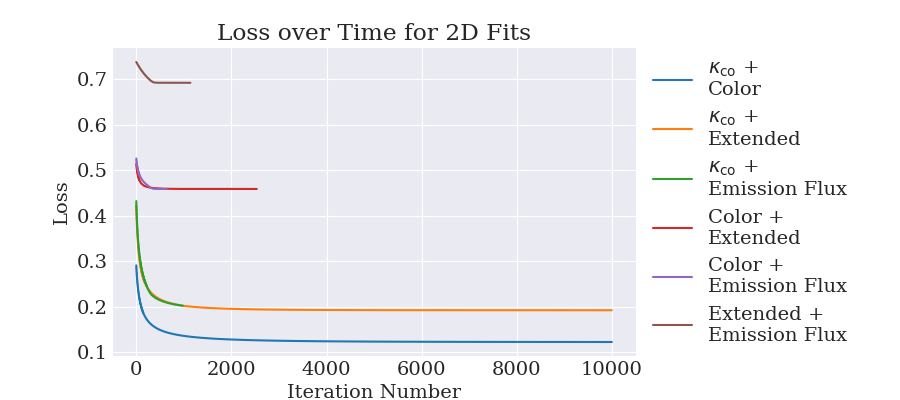
\includegraphics[width=\textwidth]{results/2d_fit_losses_constant_step.png}
    \caption{Loss value as a function of iteration number for each of the six possible combinations of two out of four features using logistic regression and a constant step size as minimization method.}
    \label{fig:losscurve_stepsize}
\end{figure}

\begin{figure}
    \centering
    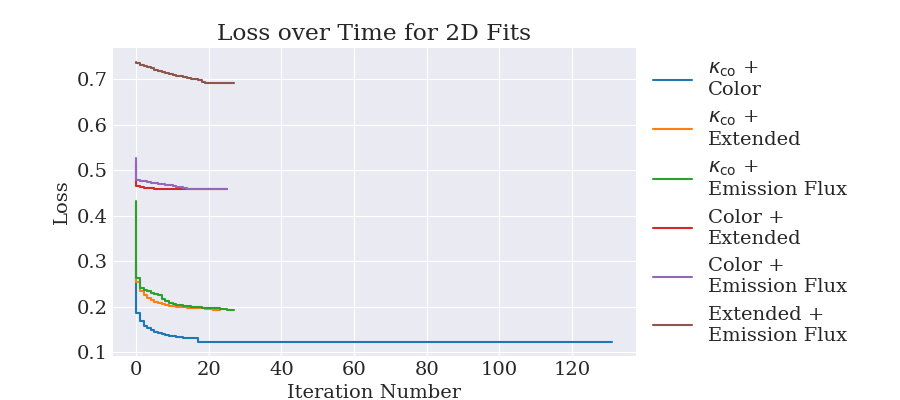
\includegraphics[width=\textwidth]{results/2d_fit_losses_line_minim.png}
    \caption{Loss value as a function of iteration number for each of the six possible combinations of two out of four features using logistic regression and line minimization as minimization method.}
    \label{fig:losscurve_linemini}
\end{figure}

We can see that under both minimization methods, all loss values converge to approximately the same values. However line minimization converges $\sim 100 - 1000$ times faster than using a learning rate of $0.1$. From these plots we can gather that the combination of $\kappa_{\mathrm{CO}}$ and color estimate is the best combination of parameters to estimate galaxy class. Meanwhile, the extended measure and the flux of the emission line tracing star formation rate appear to be a very bad combination of predictors. To get a better grasp of the distribution of the features, and the prediction capablity of our models, we plot all six of the two dimensional combinations of distributions of the features coloured by their galaxy class together with the decision boundary as learned by the logistic regression model in Figure \ref{fig:2d_line_minim_scatter}. We only plot the results of the line minimization method here.


\begin{figure}
    \centering
    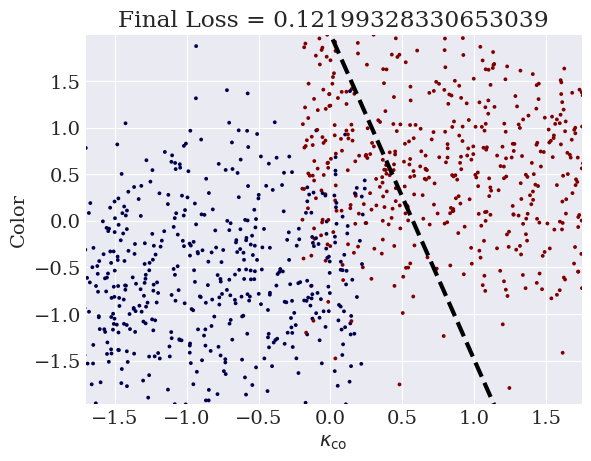
\includegraphics[width=0.48\textwidth]{results/2d_fit_line_minim_kappa_color.png}
    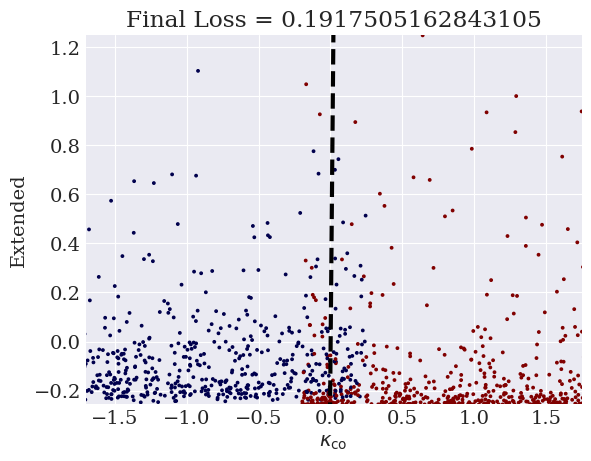
\includegraphics[width=0.48\textwidth]{results/2d_fit_line_minim_kappa_extended.png}
    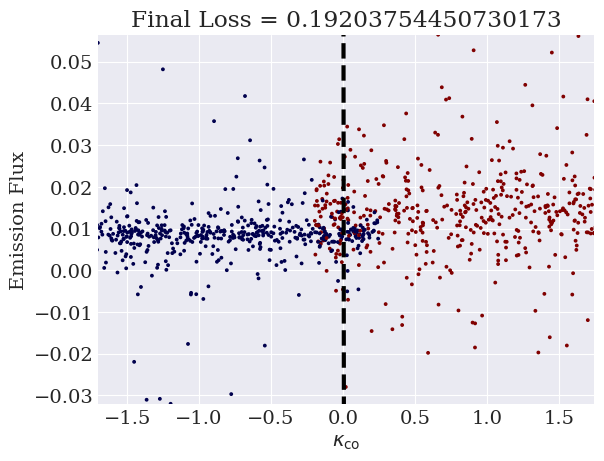
\includegraphics[width=0.48\textwidth]{results/2d_fit_line_minim_kappa_emission_flux.png}
    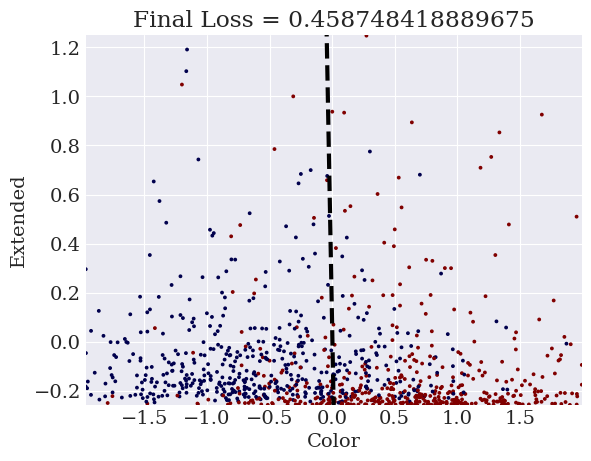
\includegraphics[width=0.48\textwidth]{results/2d_fit_line_minim_color_extended.png}
    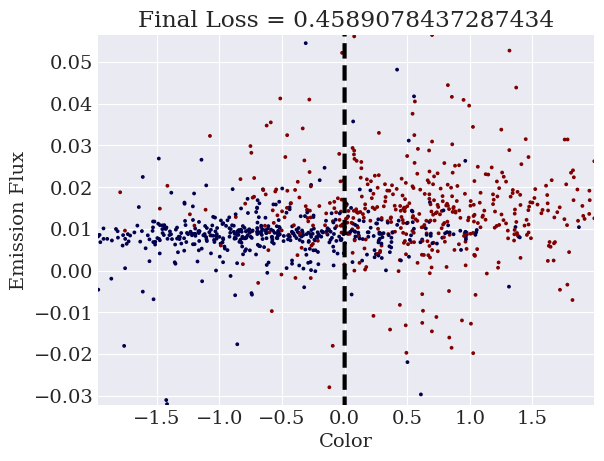
\includegraphics[width=0.48\textwidth]{results/2d_fit_line_minim_color_emission_flux.png}
    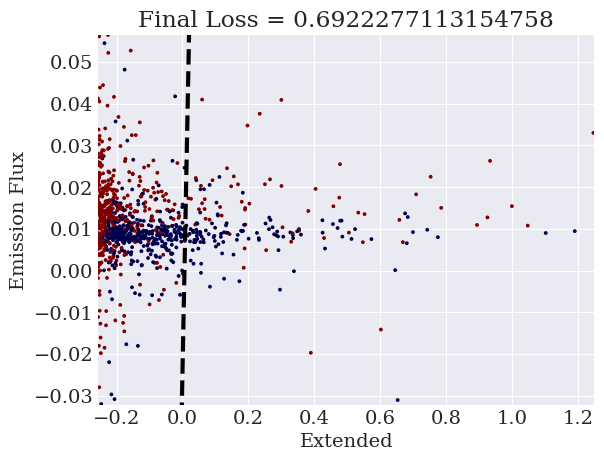
\includegraphics[width=0.48\textwidth]{results/2d_fit_line_minim_extended_emission_flux.png}
    \caption{Distributions of each combination of features with the outer 2\% cut out due to outliers. Black dashed lines indicate the decision boundary of a classification algorithm trained with logistic regression and line minimization using golden section search. The titles indicate the converged loss value.}
    \label{fig:2d_line_minim_scatter}
\end{figure}
